‫
‫‫\section*{بخش تشریحی}
‫
‫الف) شمای ستاره‌ای در زمینهٔ ذخیره و سازماندهی داده‌ها به منظور تجزیه و تحلیل و گزارش‌دهی استفاده می‌شود. مزیت اصلی استفاده از شمای ستاره‌ای آسانی  تجزیه و تحلیل داده‌هاست. در شمای ستاره‌ای، داده‌ها به دو دسته‌ی اصلی تقسیم می‌شوند: \newline
‫۱) \LR{Fact table}: این جدول حاوی اطلاعات اصلی است. \newline
‫۲) \LR{Dimension tables}: این جداول حاوی اطلاعات توصیفی در مورد ابعاد مختلف داده‌های موجود در \LR{Fact table} هستند. \newline
‫با توجه به ساختار اصلی شمای‌ ستاره‌ای، برای ذخیره‌ی اطلاعات پروازهای خارجی این شما به شکل زیر می‌باشد.
‫
‫\begin{center}
‫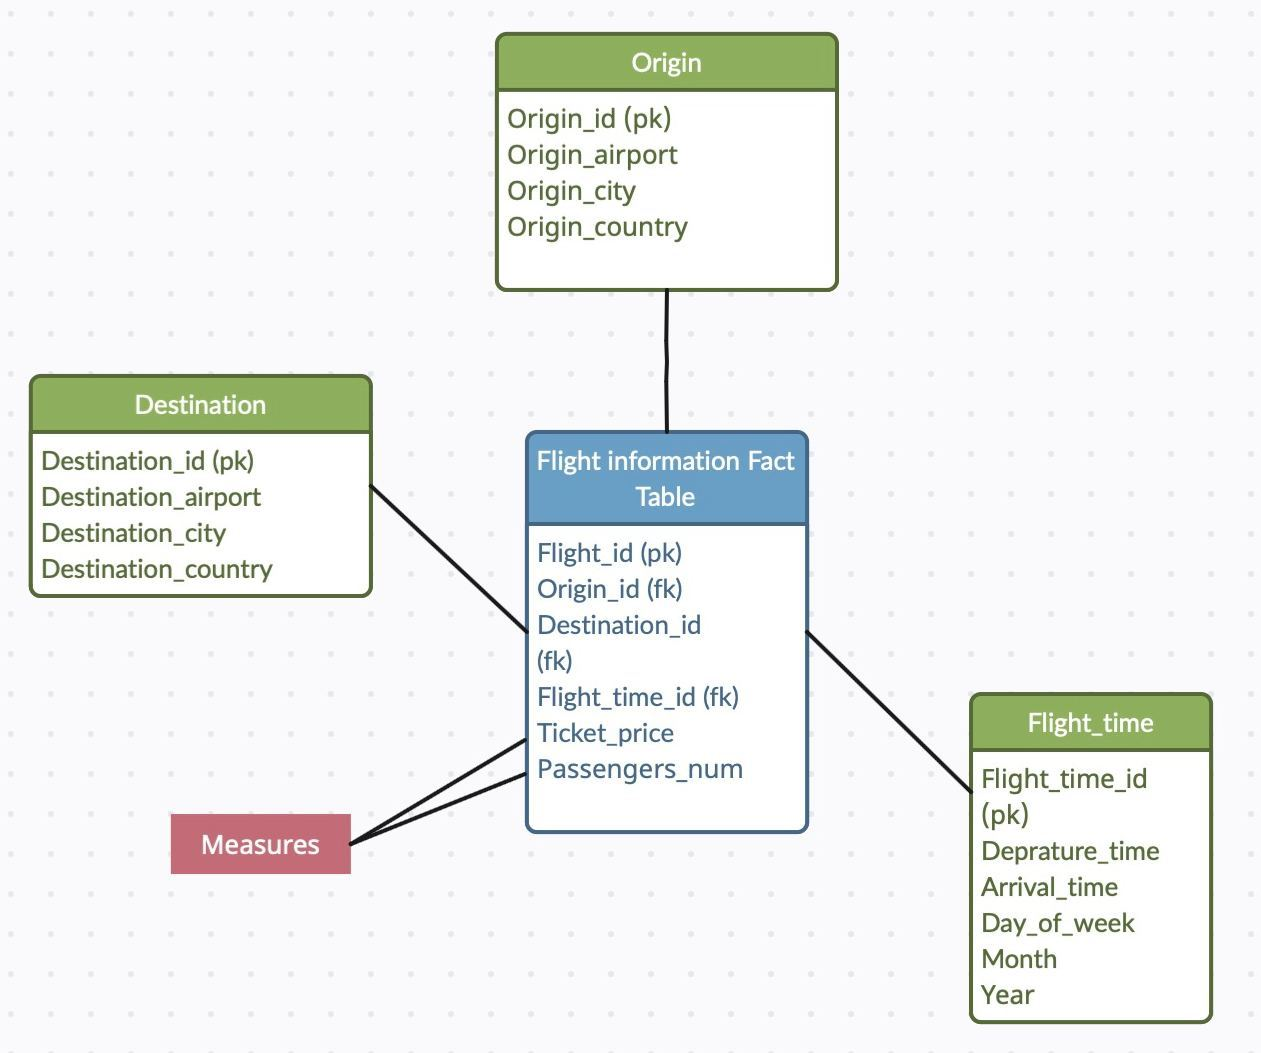
\includegraphics[scale=0.35]{figs/star_schema1.png}
‫\end{center}
‫
‫ویژگی‌های (attributes) هر کدام از بعدها در \LR{Dimension tables} خود آورده شده است. همچنین لازم به ذکر است که \LR{Flight-id} در \LR{Fact table} به عنوان کلید اصلی در نظر گرفته شده است. بسته به نیازی که تصور می‌شود می توان آن را حذف کرد یا نگه داشت. اما به صورت کلی وجود یک متغیر منحصر به فرد برای ثبت و پرس و جوی داده‌ها مناسب است.
‫\vspace{1cm}
‫
‫ب)  برای این مقایسه هر کدام از میانگین‌ها محاسبه و در پایان با یکدیگر مقایسه شده است. \newline
‫میانگین قیمت بلیط‌های تهران به میلان در خرداد ماه سال ۱۴۰۲: \newline
‫
\LR{\LR{Roll up on origin (from Origin-airport to Origin-city)} \newline
\LR{Roll up on Destination (from Destination-airport to Destination-city)} \newline
\LR{Roll up on Flight-time (from Departure-time to Month)} \newline
\LR{Dice for (Origin = “Tehran”) and (Destination = “Milan”)} \newline
\LR{Dice for (Flight-time = “Khordad”)} \newline
\LR{Roll up on Flight-time (from Month to Year)} \newline
\LR{Dice for (Flight-time = 1402)} \newline
\LR{Select AVG(Ticket-price)} \newline}

‫‫میانگین قیمت بلیط‌های تهران به آمستردام در فروردین ماه سال ۱۴۰۱: \newline
‫
\LR{\LR{Roll up on origin (from Origin-airport to Origin-city)} \newline
\LR{Roll up on Destination (from Destination-airport to Destination-city)} \newline
\LR{Roll up on Flight-time (from Departure-time to Month)} \newline
\LR{Dice for (Origin = “Tehran”) and (Destination = “Amesterdam”)} \newline
\LR{Dice for (Flight-time = “Farvardin”)} \newline
\LR{Roll up on Flight-time (from Month to Year)} \newline
\LR{Dice for (Flight-time = 1401)} \newline
\LR{Select AVG(Ticket-price)} \newline}
‫
‫\vspace{1cm}
‫
‫\hrule height .4 pt depth 0 pt width 16 cm \relax
‫
‫%------------------------------------------------------------------
‫
‫‫\section{سوال اول}
‫
‫الف)‌ برای پیمایش بهینه در chunk ها باید توجه داشت که صفحات بر اساس اندازه‌شان به ترتیب صعودی محاسبه می‌شوند. در این سوال صفحات ایجاد شده AB , AC و BC هستند که از نظر اندازه‌ی صفحه‌ها به شکل زیر می‌باشند.
‫
\begin{center}
\LR{AC < AB < BC}
\end{center}

‫با توجه به آن که BC کوچک‌تر از بقیه‌ی صفحات می‌باشد بنابراین پیمایش از این صفحه آغاز می‌شود و در ادامه در ستون بعدی در بعد A مجددا محاسبه خواهد شد.
‫
‫‫\vspace{1cm}
‫
‫ب) برای محاسبه‌ی کمترین فضایی که در حافظه‌ی اصلی نیاز است از بهینه‌ترین پیمایش در قسمت الف استفاده می‌شود. ابتدا تعداد معیارها محاسبه می‌شود. برای محاسبه‌ی تعداد آن‌ها، می‌بایست تعداد تمام cell های صفحه‌ی BC در کنار یک chunk از صفحه‌ی AC و یک ستون از صفحه‌ی AB انتخاب شود.
‫

\LR{memory = 4 * )100 * 1000 + 100 * 100000 + 100 * 100000( = 80400000  byte}

‫\vspace{1cm}
‫
‫ج) بهترین روش برای محاسبه‌ی cuboid های یک بعدی با استفاده از cuboid های دو بعدی مانند روش قبل است به این صورت که کوچکترین cuboid های دو بعدی انتخاب می‌شوند (آن‌هایی که تعداد cell کمتری دارند). به همین منظور برای cuboid های یک بعدی A , B و C بهترین حالت استفاده از cuboid های دو بعدی AB , BC و BC است.
‫
‫
‫\vspace{1cm}
‫
‫\hrule height .4 pt depth 0 pt width 16 cm \relax
‫
‫%------------------------------------------------------------------
‫
‫\section{سوال دوم}
‫
‫
‫\vspace{1cm}
‫
‫\hrule height .4 pt depth 0 pt width 16 cm \relax
‫
‫‫%------------------------------------------------------------------
‫
‫\section{سوال سوم}
‫

‫\vspace{1cm}
‫
‫\hrule height .4 pt depth 0 pt width 16 cm \relax
‫
‫‫%------------------------------------------------------------------

‫\section{سوال چهارم}

‫\vspace{1cm}
‫
‫\hrule height .4 pt depth 0 pt width 16 cm \relax
‫
‫‫%------------------------------------------------------------------
‫
‫‫‫\section*{بخش عملی}
‫
‫